\documentclass[border=10mm]{standalone}
\usepackage{tikz}
\usepackage{amsmath}
\usepackage{amssymb}
\usepackage{bm}
\usetikzlibrary{arrows.meta, fit, backgrounds, calc}

%%─── Palette ────────────────────────────────────────────────────────────────
\definecolor{tBlue}  {RGB}{52,119,196}
\definecolor{sGreen} {RGB}{56,142,60}
\definecolor{ibOrange}{RGB}{230,130,30}
\definecolor{lossRed}{RGB}{198,40,40}
\definecolor{pPurple}{RGB}{123,31,162}
\definecolor{eGold}  {RGB}{180,140,0}

%%─── Node styles ────────────────────────────────────────────────────────────
\tikzset{
  nd/.style  = {draw, rounded corners=5pt, align=center, inner sep=7pt,
                minimum width=4.0cm, minimum height=0.9cm, font=\small},
  T/.style   = {nd, draw=tBlue,   fill=tBlue!10},
  S/.style   = {nd, draw=sGreen,  fill=sGreen!10},
  ENC/.style = {nd, draw=eGold,   fill=eGold!15},
  IB/.style  = {nd, draw=ibOrange,fill=ibOrange!18},
  PL/.style  = {nd, draw=pPurple, fill=pPurple!12},
  LO/.style  = {nd, draw=lossRed, fill=lossRed!10, minimum width=3.6cm},
  %% Arrows
  Tarr/.style={-{Stealth[length=5pt]}, thick, tBlue!60, dashed},
  Sarr/.style={-{Stealth[length=5pt]}, thick, sGreen!70},
  Larr/.style={-{Stealth[length=4pt]}, thick, lossRed},
}

%% ─── Column x-centres ───────────────────────────────────────────────────────
%%  Teacher-full : x =  0
%%  Teacher-part : x =  5       (partial/indexed branch)
%%  Student      : x = 13
%%  Loss (mid)   : x =  9       (between Teacher-part and Student)
%%  Loss (right) : x = 17.6     (L_compress, right of Student)
%%  L_global     : x =  6, y = -17.2 (bottom-left)

%% ─── Row y-positions (cm, downward = more negative) ─────────────────────────
%%  Input        : y =   0
%%  Encoder      : y =  -2.5
%%  CLS          : y =  -5.0
%%  Pool         : y =  -7.5
%%  Pooled repr  : y = -10.0
%%  IB head      : y = -12.8   (taller node)
%%  MLP          : y = -15.6
%%  Z_proj       : y = -17.9   (also y for L_global)

\begin{document}
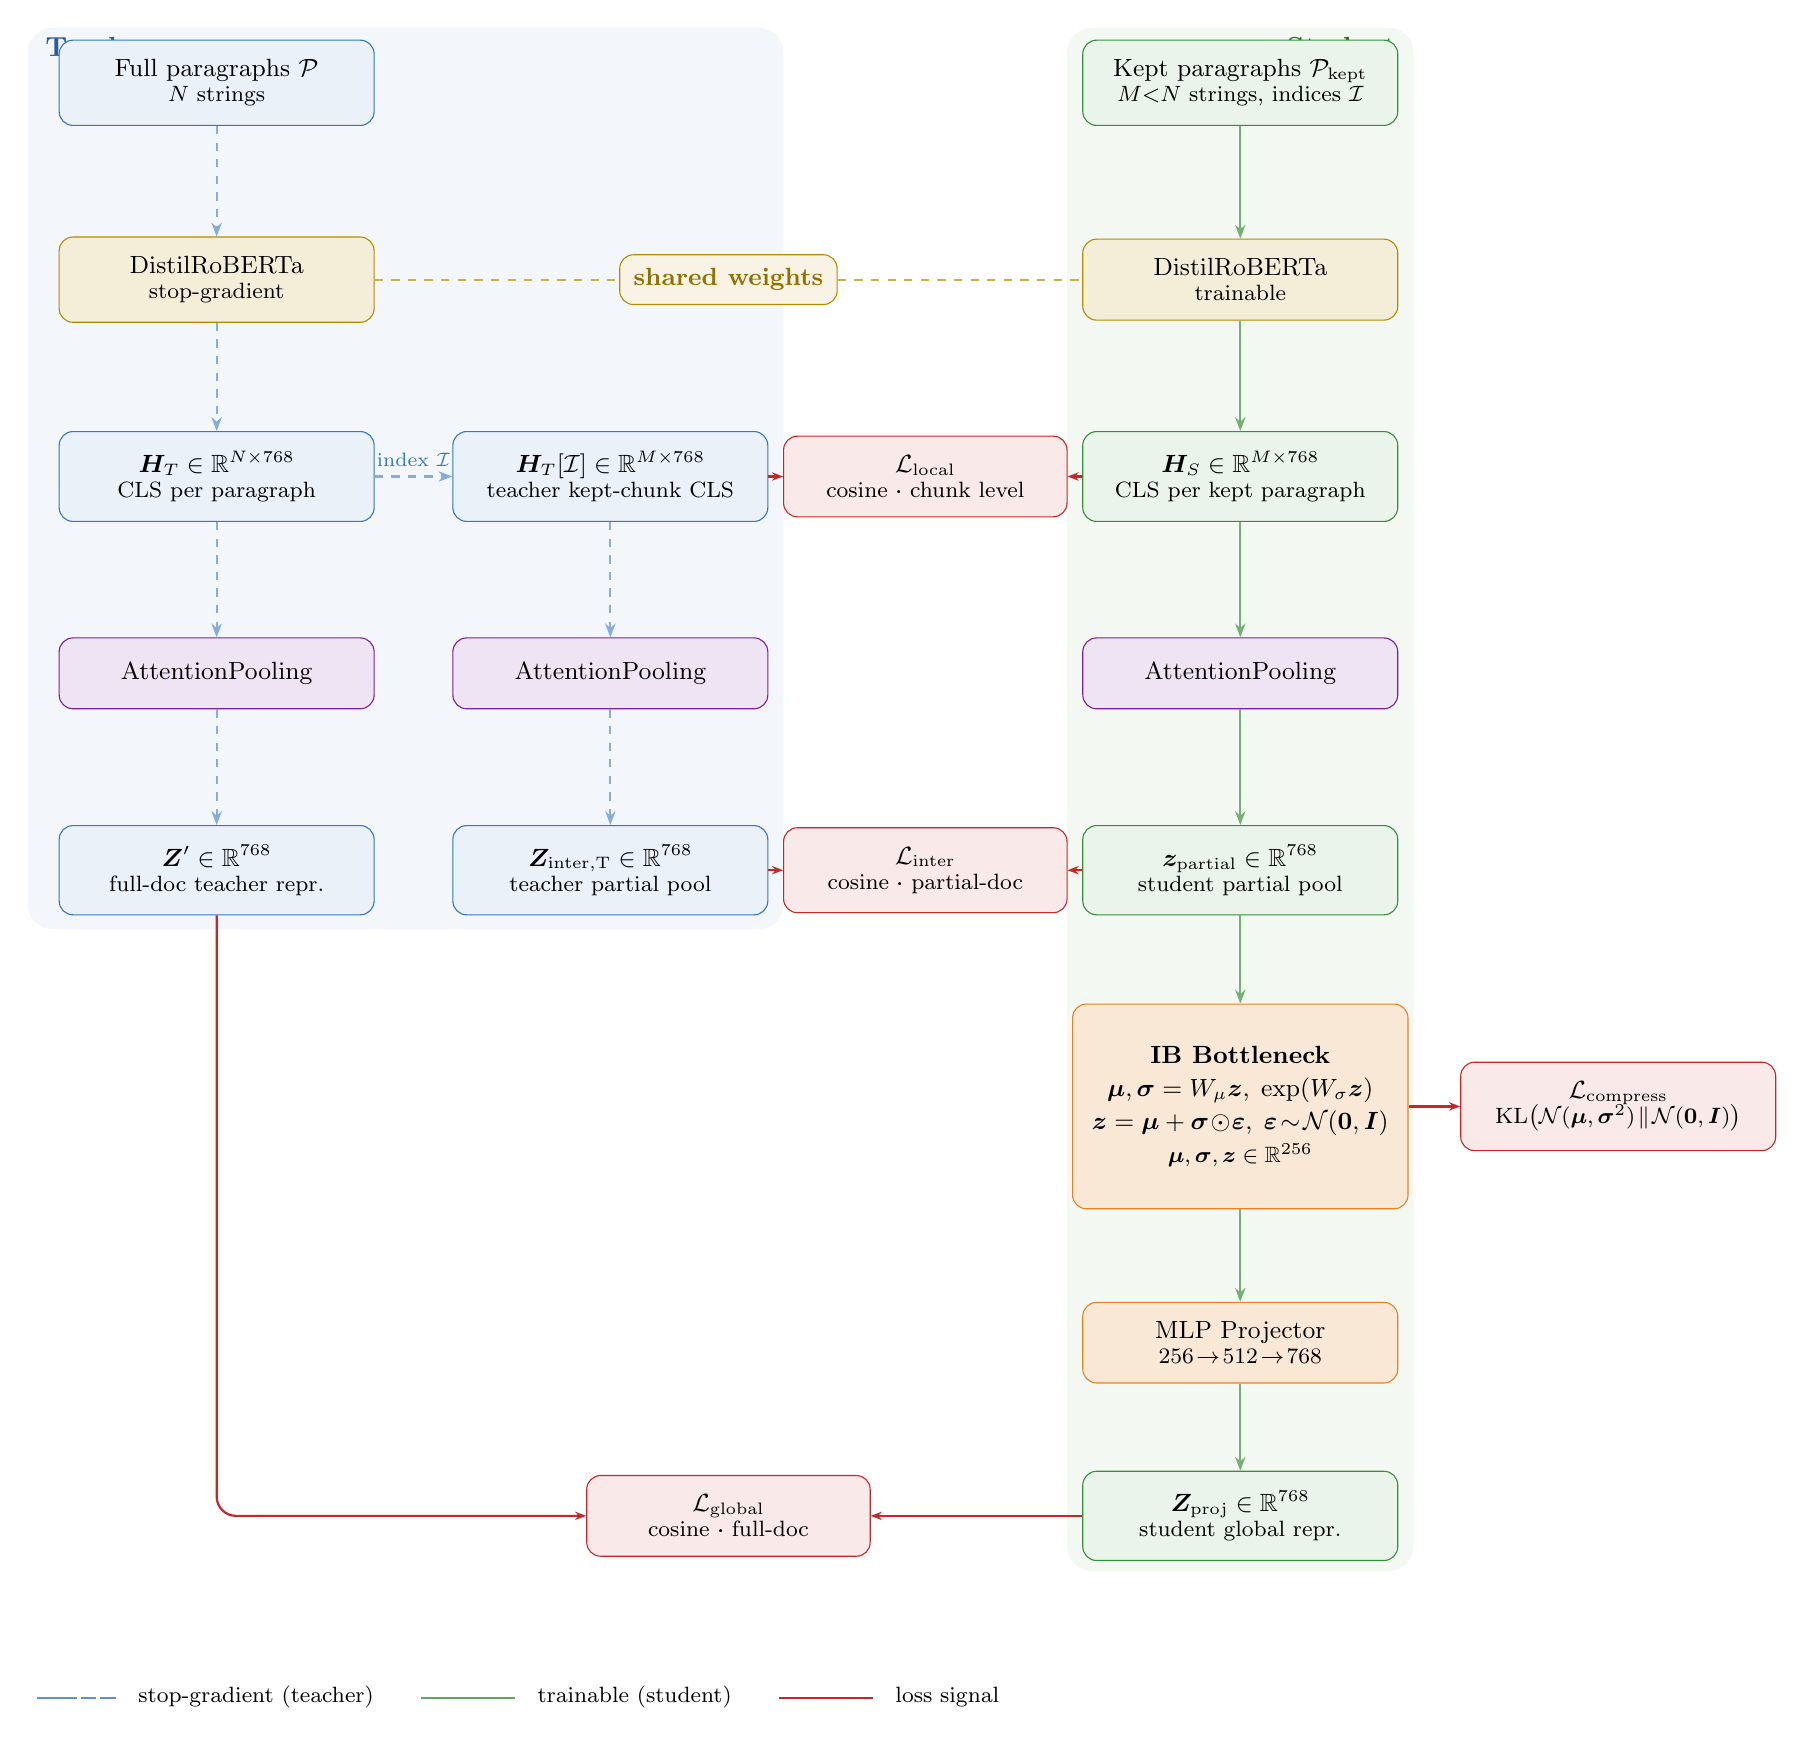
\begin{tikzpicture}

%% ═══════════════════════════════════════════════════════
%%  TEACHER – full-document track (left column, x = 0)
%% ═══════════════════════════════════════════════════════

\node[T]   (t_in)  at ( 0,   0  ) {Full paragraphs $\mathcal{P}$\\[-2pt]
                                    \footnotesize $N$ strings};

\node[ENC] (t_enc) at ( 0,  -2.5) {DistilRoBERTa\\[-2pt]
                                    \footnotesize stop-gradient};

\node[T]   (t_cls) at ( 0,  -5.0) {$\bm{H}_T\in\mathbb{R}^{N\times768}$\\[-2pt]
                                    \footnotesize CLS per paragraph};

\node[PL]  (t_pl)  at ( 0,  -7.5) {AttentionPooling};

\node[T]   (t_zp)  at ( 0, -10.0) {$\bm{Z}'\in\mathbb{R}^{768}$\\[-2pt]
                                    \footnotesize full-doc teacher repr.};

\draw[Tarr] (t_in) -- (t_enc);
\draw[Tarr] (t_enc)--(t_cls);
\draw[Tarr] (t_cls)--(t_pl);
\draw[Tarr] (t_pl) --(t_zp);


%% ═══════════════════════════════════════════════════════
%%  TEACHER – partial (indexed) track (x = 5)
%% ═══════════════════════════════════════════════════════

\node[T]  (t_ki)  at ( 5,  -5.0) {$\bm{H}_T[\mathcal{I}]\in\mathbb{R}^{M\times768}$\\[-2pt]
                                   \footnotesize teacher kept-chunk CLS};

\node[PL] (t_kpl) at ( 5,  -7.5) {AttentionPooling};

\node[T]  (t_zit) at ( 5, -10.0) {$\bm{Z}_{\mathrm{inter,T}}\in\mathbb{R}^{768}$\\[-2pt]
                                   \footnotesize teacher partial pool};

%% Branch: H_T → H_T[I]
\draw[Tarr] (t_cls.east) --
            node[above, font=\scriptsize, tBlue]{index $\mathcal{I}$}
            (t_ki.west);
\draw[Tarr] (t_ki) --(t_kpl);
\draw[Tarr] (t_kpl)--(t_zit);


%% ═══════════════════════════════════════════════════════
%%  STUDENT (right column, x = 13)
%% ═══════════════════════════════════════════════════════

\node[S]   (s_in)  at (13,   0  ) {Kept paragraphs $\mathcal{P}_{\mathrm{kept}}$\\[-2pt]
                                    \footnotesize $M{<}N$ strings, indices $\mathcal{I}$};

\node[ENC] (s_enc) at (13,  -2.5) {DistilRoBERTa\\[-2pt]
                                    \footnotesize trainable};

\node[S]   (s_cls) at (13,  -5.0) {$\bm{H}_S\in\mathbb{R}^{M\times768}$\\[-2pt]
                                    \footnotesize CLS per kept paragraph};

\node[PL]  (s_pl)  at (13,  -7.5) {AttentionPooling};

\node[S]   (s_zpt) at (13, -10.0) {$\bm{z}_{\mathrm{partial}}\in\mathbb{R}^{768}$\\[-2pt]
                                    \footnotesize student partial pool};

\node[IB, minimum height=2.6cm]
           (s_ib)  at (13, -13.0) {\textbf{IB Bottleneck}\\[1pt]
                                    $\bm{\mu},\bm{\sigma}
                                     = W_\mu\bm{z},\;\exp(W_\sigma\bm{z})$\\[1pt]
                                    $\bm{z}
                                     =\bm{\mu}+\bm{\sigma}\!\odot\!\bm{\varepsilon},\;
                                      \bm{\varepsilon}\!\sim\!\mathcal{N}(\bm{0},\bm{I})$\\[1pt]
                                    \footnotesize
                                    $\bm{\mu},\bm{\sigma},\bm{z}\in\mathbb{R}^{256}$};

\node[IB]  (s_mlp) at (13, -16.0) {MLP Projector\\[-2pt]
                                    \footnotesize $256\!\to\!512\!\to\!768$};

\node[S]   (s_zpj) at (13, -18.2) {$\bm{Z}_{\mathrm{proj}}\in\mathbb{R}^{768}$\\[-2pt]
                                    \footnotesize student global repr.};

\draw[Sarr] (s_in) --(s_enc);
\draw[Sarr] (s_enc)--(s_cls);
\draw[Sarr] (s_cls)--(s_pl);
\draw[Sarr] (s_pl) --(s_zpt);
\draw[Sarr] (s_zpt)--(s_ib);
\draw[Sarr] (s_ib) --(s_mlp);
\draw[Sarr] (s_mlp)--(s_zpj);


%% ═══════════════════════════════════════════════════════
%%  LOSS NODES
%% ═══════════════════════════════════════════════════════

%% L_local  ─ chunk level ─────────────────────────────
\node[LO] (l_loc) at (9, -5.0) {$\mathcal{L}_{\mathrm{local}}$\\[-2pt]
                                  \footnotesize cosine · chunk level};
\draw[Larr] (t_ki.east) --(l_loc.west);
\draw[Larr] (s_cls.west)--(l_loc.east);

%% L_inter  ─ partial-doc level ───────────────────────
\node[LO] (l_int) at (9,-10.0) {$\mathcal{L}_{\mathrm{inter}}$\\[-2pt]
                                  \footnotesize cosine · partial-doc};
\draw[Larr] (t_zit.east)--(l_int.west);
\draw[Larr] (s_zpt.west)--(l_int.east);

%% L_compress  ─ KL bottleneck ────────────────────────
\node[LO, minimum width=4.0cm]
      (l_cmp) at (17.8,-13.0) {$\mathcal{L}_{\mathrm{compress}}$\\[-2pt]
                                \footnotesize $\mathrm{KL}\bigl(
                                \mathcal{N}(\bm\mu,\bm\sigma^2)
                                \!\parallel\!\mathcal{N}(\bm 0,\bm I)\bigr)$};
\draw[Larr] (s_ib.east)--(l_cmp.west);

%% L_global  ─ full-doc level ─────────────────────────
%%   Z'    is at (  0, -10.0)
%%   Z_proj is at ( 13, -18.2)
%%   Place loss node at (6.5, -18.2);
%%   route from Z': south → (0,-18.2) → loss.west
\node[LO] (l_glb) at (6.5,-18.2) {$\mathcal{L}_{\mathrm{global}}$\\[-2pt]
                                    \footnotesize cosine · full-doc};
\draw[Larr] (s_zpj.west)--(l_glb.east);
\draw[Larr, rounded corners=7pt]
     (t_zp.south) -- (0,-18.2) -- (l_glb.west);


%% ═══════════════════════════════════════════════════════
%%  SHARED ENCODER BADGE
%% ═══════════════════════════════════════════════════════
\node[draw=eGold, fill=eGold!10, rounded corners=5pt,
      font=\small\bfseries, text=eGold!80!black, inner sep=5pt]
     (badge) at (6.5,-2.5) {shared weights};

%% dashed connectors from badge to each encoder
\draw[eGold!70, dashed, thick] (t_enc.east) -- (badge.west);
\draw[eGold!70, dashed, thick] (badge.east) -- (s_enc.west);


%% ═══════════════════════════════════════════════════════
%%  BACKGROUND PANELS
%% ═══════════════════════════════════════════════════════
\begin{scope}[on background layer]
  %% Teacher panel  (covers both teacher columns)
  \fill[tBlue!6, rounded corners=9pt]
    (-2.4, 0.7) rectangle (7.2,-10.75);
  \node[tBlue!80!black, font=\bfseries, anchor=north west]
       at (-2.3,0.7) {Teacher};

  %% Student panel
  \fill[sGreen!6, rounded corners=9pt]
    (10.8, 0.7) rectangle (15.2,-18.9);
  \node[sGreen!80!black, font=\bfseries, anchor=north east]
       at (15.1,0.7) {Student};
\end{scope}


%% ═══════════════════════════════════════════════════════
%%  LEGEND
%% ═══════════════════════════════════════════════════════
\node[font=\footnotesize, anchor=west, align=left]
     at (-2.4,-20.5) {%
  \textcolor{tBlue!80}{\rule[0.4ex]{0.5cm}{0.5pt}%
  \,\rule[0.4ex]{0.2cm}{0.5pt}\,\rule[0.4ex]{0.2cm}{0.5pt}}
  \; stop-gradient (teacher)\qquad
  \textcolor{sGreen!80}{\rule[0.4ex]{1.2cm}{0.5pt}}
  \; trainable (student)\qquad
  \textcolor{lossRed}{\rule[0.4ex]{1.2cm}{0.5pt}}
  \; loss signal
};

\end{tikzpicture}
\end{document}